% \chapter{Giới thiệu}
% \label{chap:chap1-introduce}

% Tại chương này, tác giả giới thiệu cấu trúc thư mục của dự án, giải thích các cài đặt, một số lưu ý trong quá trình sử dụng. Chương này cũng như báo cáo này không giới thiệu các cú pháp cơ bản như gõ phương trình, tạo bảng đơn giản, chèn hình ảnh.

% \section{Cấu trúc thư mục}

% \indent Hình \ref{fig:chap1-project-directory} mô tả cấu trúc thư mục của dự án. Thư mục \textbf{chapters} lưu các thành phần văn bản chính của dự án. Trong thư mục này chia làm ba thư mục, \textbf{\textit{back}} tương ứng với các phụ lục phía sau báo cáo.

% \begin{figure}
%     \centering
%     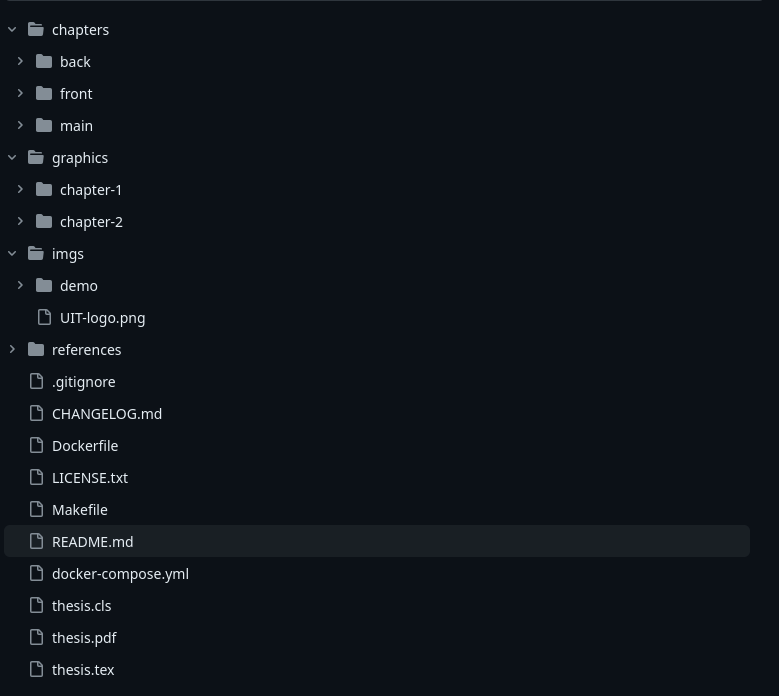
\includegraphics[scale=0.5]{chapter1/chap1-project-directory.png}
%     \caption{Cấu trúc thư mục của dự án}
%     \label{fig:chap1-project-directory}
% \end{figure}


% Thư mục \textbf{\textit{front}} tương ứng với các trang thông tin hội đồng chấm tốt nghiệp, lời cảm ơn, danh mục từ viết tắt... Thư mục \textbf{\textit{main}} chứa các chương của báo cáo. Báo cáo đánh số thứ tự riêng cho phần \textit{\textbf{front}}, trong khi phần các chương chính và phần phụ lục được đánh số giống nhau. Báo cáo đánh số trang bắt đầu từ trang tóm tắt, chữ số Ả-rập, bắt đầu bằng 1.

% Thư mục \textbf{\textit{graphics}} chứa hình ảnh được chèn vào báo cáo. Tương ứng với mỗi chương sẽ có 1 thư mục hình ảnh của chương đó.

% Thư mục \textbf{\textit{imgs}} là thư mục chứa hình ảnh của dự án, nó bao gồm các logo, watermark hoặc hình ảnh phục vụ cho document trên github. Hình chèn vào báo cáo không được lưu trong thư mục này.

% Thư mục \textbf{\textit{references}} chứa các file chỉ mục tài liệu tham khảo. Tương tự như mỗi chapter một file .tex, nó cũng có riêng một file .bib để chỉ rõ các tài liệu tham khảo nào được sử dụng trong chuong nào.

% File \textbf{\textit{thesis.cls}} là file quy định các câu lệnh, mức chỉ mục đánh số hình ảnh, bảng biểu, phần, chương. Quy định header và footer, trang  bìa.... Chi tiết xem trong file. Hãy chắc chắn rằng bạn hiểu rõ tất cả nếu muốn thay đổi gì trong file này.

% File \textbf{\textit{thesis.tex}} là file quy định cấu trúc báo cáo, chương nào trước, chương nào sau, quy định thư mục hình ảnh chèn trong báo cáo. Nó quy định thông tin người báo cáo thông qua các câu lệnh được quy định trong file .cls. 

% \section{Thay đổi các biến khi sử dụng}

% Hai bìa của luận văn được tự động tạo bởi latex. Vì vậy, có các biến được quy định để đảm nhiệm nó. Các biến cần thay đổi được đặt tại thư mục gốc, tập tin \textit{thesis.tex}, được thể hiện trong hình \ref{fig:chap1-information-variable}.

% \begin{figure}
%     \centering
%     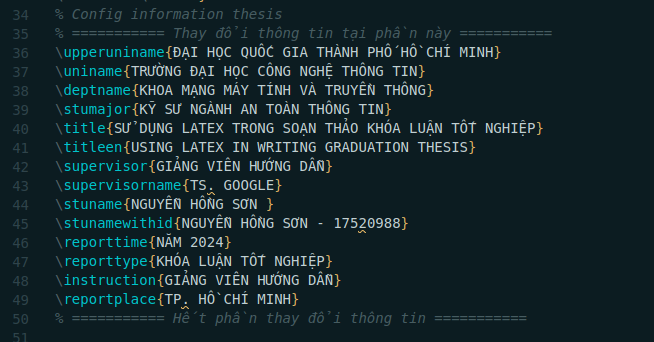
\includegraphics[scale=0.7]{chapter1/chap1-information-variable.png}
%     \caption{Phần thay đổi thông tin trang bìa}
%     \label{fig:chap1-information-variable}
% \end{figure}

% Các phần tiếp theo, quy định các nội dung được thêm vào báo cáo chính. Nếu một tập tin xuất hiện trong thư mục chapters nhưng không được khai báo bằng lệnh \textit{include} thì cũng không xuất hiện trong báo cáo. Vậy nên các chương mới bắt buộc phải được khai báo trong \textit{thesis.tex}. Các phần tài liêu tham khảo cũng được hiểu tương tự.

\chapter{Tổng quan}
\label{chap:chap1}
\section{Bối cảnh và bài toán nghiên cứu}
Trong bối cảnh công nghệ blockchain ngày càng phát triển, nhu cầu về mở rộng \cite{song2024advancing} và cải thiện hiệu suất giao dịch đang ngày càng trở nên cấp thiết  \cite{etherscan_pending} \cite{etherscan_token}. Các giải pháp để cải thiện vấn đề này đã được đề xuất như sharding, side-chains, state-channels,... Trong số đó, ZK-Rollup đã được nghiên cứu và ứng dụng rộng rãi như một giải pháp để cải thiện khả năng mở rộng blockchain bằng layer 2 hiệu quả. Các giải pháp ZK-Rollup đã được triển khai và sử dụng phổ biến trong những năm gần đây như ZKSync Era, Starknet, Polygon zkEVM \cite{chaliasos2024analyzing},... đã cho thấy ZK-Rollup là giải pháp tiềm năng để nghiên cứu, tối ưu và phát triển nhắm đến mục tiêu chính là cải thiện khả năng mở rộng cho các blockchain layer 1 như Ethereum.
ZK-Rollups tổng hợp nhiều giao dịch riêng lẻ ngoài chuỗi thành một lô duy nhất \cite{thibault2022blockchain}. Sau đó, một bằng chứng không tri thức (ZKP - Zero Knowledge Proof) về tính hợp lệ của các giao dịch này được tạo ra, và chỉ có bằng chứng này, cùng với dữ liệu giao dịch đã nén, được đăng tải lên lớp 1 để xác minh. Phương pháp này giảm thiểu đáng kể dữ liệu và tính toán trên chuỗi, từ đó tăng cường thông lượng giao dịch và giảm phí gas. Điều này không chỉ làm tăng tốc độ giao dịch mà còn đảm bảo an toàn bằng cách kế thừa các đảm bảo bảo mật của lớp 1 thông qua các bằng chứng hợp lệ \cite{saif2024survey}.
Mặc dù là giải pháp đầy hứa hẹn, nhưng việc triển khai thực tiễn ZK-Rollup đang gặp phải một số thách thức đáng kể, chủ yếu liên quan đến sự phức tạp cố hữu của các mạch bằng chứng không kiến thức \cite{zhou2024leveraging}. Việc xây dựng các mạch ZK (zero-knowledge) một cách thủ công rất phức tạp và dễ mắc lỗi \cite{chaliasos2024sok}. Hiệu suất của các hệ thống ZKP, đặc biệt là quy trình tạo bằng chứng, hiện đang là một trong những mối quan tâm lớn khi nghiên cứu về bằng chứng không kiến thức. Với các mạch phức tạp, số lượng các ràng buộc trở thành một trong những yếu tố gây cản trở, ảnh hưởng đến nhiều khía cạnh của quy trình tạo bằng chứng, chẳng hạn như thời gian biên dịch mạch, thời gian tạo bằng chứng và mức tiêu thụ bộ nhớ cần thiết để thực hiện những tác vụ này \cite{belles2022circom}.
Mặc dù đã có nhiều nỗ lực nhằm tăng tốc tính toán bằng chứng, những tiến bộ trong việc tối ưu hóa quy trình tạo bằng chứng vẫn còn hạn chế, cản trở đến hiệu suất tổng thể. Các nghiên cứu về chủ đề này thường tập trung vào việc phát triển các hệ thống tạo bằng chứng, đề xuất các hệ thống ZKP mới \cite{gong2022analysis} như STARK \cite{ben2018scalable}, Bulletproof \cite{bunz2018bulletproofs} và Plonk \cite{gabizon2019plonk}. Tuy nhiên, vấn đề thực tiễn đầu tiên mà các nhà phát triển phải đối mặt nằm trong hệ thống ràng buộc và trình biên dịch. Tập trung vào các cờ tối ưu của trình biên dịch Circom, một công cụ quan trọng và phổ biến để quản lý độ phức tạp và hiệu suất của mạch, sẽ trực tiếp giải quyết khoảng trống này ở cấp độ cơ bản của việc thiết kế và triển khai mạch.

Việc hiểu rõ tác động của các cờ tối ưu hóa này sẽ cung cấp kiến thức nền tảng quan trọng, giúp các nhà phát triển đưa ra quyết định tốt hơn ngay từ giai đoạn thiết kế và triển khai mạch, trước khi xem xét các tối ưu hóa phức tạp hơn ở cấp độ hệ thống (như độ trễ mạng, thiết kế hệ thống hoặc các chiến lược tối ưu hệ thống ZKP chuyên sâu hơn) \cite{liang2025sok}.

Nhằm giải quyết những thách thức trên, khoá luận này đề xuất nghiên cứu đề tài ``NÂNG CAO HIỆU SUẤT GIAO DỊCH ERC-20 TRÊN ZK-ROLLUP THÔNG QUA XỬ LÝ RÀNG BUỘC MẠCH GROTH16''. Đề tài này tập trung vào hai mục tiêu chính:
\begin{enumerate}
    \item \textbf{Phân tích sự ảnh hưởng của ràng buộc đến các giai đoạn trong quá trình tạo bằng chứng không kiến thức}: Nghiên cứu định lượng sự ảnh hưởng của số lượng ràng buộc đến thời gian tạo bằng chứng không kiến thức, và sự đánh đổi giữa thời gian biên dịch với số lượng ràng buộc được tối ưu khi áp dụng các cờ tối ưu của Circom.
    \item \textbf{Cung cấp khung gợi ý sử dụng cờ tối ưu hoá Circom}: Đề xuất một khung gợi ý để sử dụng các cờ tối ưu hoá Circom trong thực tế nhằm cân bằng thời gian biên dịch mạch và hiệu suất tạo bằng chứng không kiến thức trong quá trình phát triển mạch không kiến thức.
\end{enumerate}
Với những mục tiêu được đề cập ở trên, khoá luận này hy vọng sẽ cung cấp được một cái nhìn cụ thể, trực quan hơn về cách Circom tối ưu hoá ràng buộc của mạch nhằm tăng hiệu suất tạo bằng chứng không kiến thức. Đồng thời hỗ trợ giải quyết nhu cầu thực tế trong phát triển hệ thống ZK-Rollup. Việc quản lý tối ưu hóa ràng buộc một cách hiệu quả không chỉ giảm thiểu chi phí tạo bằng chứng mà còn ảnh hưởng trực tiếp đến chu kỳ lặp khi phát triển ứng dụng, tạo điều kiện thuận lợi cho việc tích hợp các mạch không kiến thức vào các ứng dụng blockchain. Qua đó, hỗ trợ việc áp dụng rộng rãi ZK-Rollup trong các môi trường blockchain nhạy cảm về chi phí và yêu cầu cao về hiệu suất.

\section{Mục tiêu}

Công nghệ bằng chứng không kiến thức khi được áp dụng vào các ứng dụng thực tế như ZK-Rollup luôn gặp phải vấn đề cố hữu là kích thước mạch lớn và thời gian tạo bằng chứng dài do các hoạt động mật mã phức tạp trong các thuật toán đại số. Do đó, khoá luận này sẽ tập trung nghiên cứu vào tác động của ràng buộc đến thời gian tạo bằng chứng không kiến thức, cũng như những đánh đổi về thời gian biên dịch để tối ưu mạch chứng minh không kiến thức nhằm giảm số lượng ràng buộc. Từ đó đưa ra một khung gợi ý sử dụng cờ tối ưu hoá Circom nhằm tăng hiệu quả phát triển ứng dụng sử dụng bằng chứng không kiến thức như ZK-Rollup trong thực tế. 
Cụ thể, khoá luận này đề ra các mục tiêu cụ thể như sau:
\begin{enumerate}
    \item \textbf{Khảo sát và phân tích các phương pháp hiện tại}: Bắt đầu quá trình nghiên cứu, khoá luận sẽ tiến hành một khảo sát toàn diện về những phương pháp giúp cải tiến hiệu suất tạo bằng chứng không kiến thức cho hệ thống zk-SNARKs. Từ đó thu hẹp phạm vi lại hướng đến việc cải thiện hiệu suất tạo bằng chứng không kiến thức thông qua tối ưu hoá ràng buộc trong mạch. Mục tiêu của giai đoạn này là tìm hiểu về các giải pháp tối ưu cho việc tạo bằng chứng không kiến thức, tìm ra khoảng trống nghiên cứu nhằm nghiên cứu đưa ra cách giải quyết hiệu quả cho khoảng trống này (ví dụ các công trình như
    \cite{albert2022distilling, ben2018scalable, bunz2018bulletproofs, ernstberger2024zk,gabizon2019plonk,gong2022analysis, el2024evaluating,  pailoor2023automated}).
    \item \textbf{Phân tích và đánh giá định lượng tác động của các cờ tối ưu hóa ràng buộc khác nhau (--O0, --O1, --O2) trong trình biên dịch Circom đối với hiệu suất của hệ thống ZK-Rollup mô phỏng giao dịch ERC-20}: Tiếp theo, khoá luận sẽ tập trung vào việc phân tích các dữ liệu lấy được từ quá trình thực nghiệm. Quá trình này bao gồm việc đo lường và so sánh:
    \begin{itemize}
        \item Số lượng ràng buộc tổng thể, số lượng ràng buộc tuyến tính và phi tuyến được tạo ra.
        \item Thời gian cần thiết để biên dịch mạch (compilation time).
        \item Thời gian cần thiết để tạo bằng chứng không tri thức (proving time) sử dụng backend Groth16.
        \item Thời gian và chi phí để xác minh bằng chứng không kiến thức trên blockchain lớp 1.
    \end{itemize}
    \item \textbf{Khảo sát mối quan hệ giữa các mức tối ưu hóa ràng buộc, kích thước lô giao dịch, và các chỉ số hiệu suất đã nêu}: Xác định các xu hướng và sự đánh đổi giữa thời gian biên dịch và thời gian tạo bằng chứng khi thay đổi các cờ tối ưu khác nhau.

    \item \textbf{Phân tích cơ chế hoạt động của cờ tối ưu hóa --O2 trong Circom, đặc biệt là cách nó loại bỏ các ràng buộc tuyến tính và ảnh hưởng đến cấu trúc ràng buộc phi tuyến còn lại}: Đánh giá hiệu quả của việc tập trung tài nguyên tính toán vào các ràng buộc phi tuyến.

    \item \textbf{Đề xuất một khung hướng dẫn thực tiễn cho việc lựa chọn cờ tối ưu hóa Circom phù hợp}:  Khung này sẽ dựa trên các kết quả thực nghiệm và xem xét các yếu tố như giai đoạn phát triển của dự án (phát triển, kiểm thử, sản xuất), tần suất cập nhật mạch, và khối lượng bằng chứng dự kiến cần tạo. Góp phần vào việc giảm thiểu chi phí triển khai, rút ngắn chu kỳ phát triển, và thúc đẩy việc áp dụng rộng rãi công nghệ ZK-Rollup trong các ứng dụng blockchain thực tế.
\end{enumerate}
\section{Phạm vi đề tài và đối tượng nghiên cứu}
Đề tài sẽ tập trung phân tích mức độ hiệu quả cũng như các đánh đổi khi áp dụng các mức tối ưu hoá ràng buộc mạch của Circom. Từ đó đánh giá sự ảnh hưởng của các thông số ghi lại được trong quá trình tạo bằng chứng không kiến thức và đề xuất khung hướng dẫn sử dụng cờ tối ưu Circom phù hợp với từng giai đoạn phát triển mạch bằng chứng không kiến thức trong ZK-Rollup thực tế.
Đối tượng nghiên cứu của đề tài bao gồm:

\begin{itemize}
    \item \textbf{Hệ thống ZK-Rollup}: Tập trung vào triển khai thực nghiệm với hệ thống ZK-Rollup mô phỏng với tác vụ chính là giao dịch token ERC-20.
    \item \textbf{Công cụ và cơ chế tối ưu hoá ràng buộc cho mạch chứng minh không kiến thức}: Phạm vi nghiên cứu được giới hạn trong việc phân tích và đánh giá tác động của các cờ tối ưu hóa ràng buộc (-O0, -O1, và -O2) của trình biên dịch Circom.
    \item \textbf{Hệ thống chứng minh không kiến thức}: Các thí nghiệm và phân tích sẽ được thực hiện dựa trên hệ thống bằng chứng không kiến thức Groth16, một trong những hệ thống zk-SNARK phổ biến nhất hiện nay.
    \item \textbf{Giải pháp sử dụng các mức tối ưu hoá hiệu quả}: Đưa ra khung gợi ý sử dụng các mức tối ưu hoá phù hợp khi phát triển mạch bằng chứng không kiến thức khi xây dựng ZK-Rollup.
\end{itemize}

\section{Cấu trúc báo cáo khoá luận}
Khoá luận này có cấu trúc gồm 6 chương, được trình bày như sau: 
\begin{itemize}
    \item \textbf{Chương \ref{chap:chap1} - Tổng quan:} Trình bày bối cảnh, mục đích, đối tượng và phạm vi nghiên cứu của đề tài.
    \item \textbf{Chương \ref{chap:chap2} - Nghiên cứu liên quan:} Trình bày các công trình nghiên cứu liên quan và khoảng trống nghiên cứu.
    \item \textbf{Chương \ref{chap:chap3} - Cơ sở lý thuyết:} Cung cấp kiến thức về blockchain, ZK-Rollup, giao dịch ERC-20, kiến thức liên quan về hệ thống chứng minh không kiến thức được sử dụng, trình biên dịch Circom và các cờ tối ưu hoá.
    \item \textbf{Chương \ref{chap:chap4} - Phương pháp đề xuất và công cụ hỗ trợ:} Trình bày chiến lược tối ưu hoá ràng buộc theo vòng đời phát triển mạch ZKP sử dụng Circom, gọi tắt là ZCLS (ZK Circuit Lifecycle Strategy), cùng các bước thực nghiệm và công cụ CirMetrics được thiết kế để hỗ trợ triển khai chiến lược này.
    \item \textbf{Chương \ref{chap:chap5} - Kết quả thực nghiệm và đánh giá:} Trình bày kết quả thực nghiệm, thảo luận và đề xuất khung gợi ý sử dụng cờ tối ưu của trình biên dịch Circom.
    % \item \textbf{Chương \ref{chap:chap6}} - \textbf{CirMetrics:} Giới thiệu hệ thống hỗ trợ theo dõi các thống số của mạch ZK, hỗ trợ các nhà phát triển quản lí mạch trong quá trình xây dựng mạch ZK.
    \item \textbf{Chương \ref{chap:chap6} - Kết luận và hướng phát triển:} Trình bày những kết quả đạt được, những đóng góp và đề xuất mới. 
    \item \textbf{Tài liệu tham khảo:} Các công trình nghiên cứu được trích dẫn trong khoá luận.
\end{itemize}